\chapter{Fundamentação}
(...)

%% 1 ::: Introdução
%% 1.1
\section{Problemas de Agendamento}
%% Interlúdio do [Problemas de Agendamento] %%
Problemas de agendamento são muito comuns atualmente, pois estão diretamente presentes em diversos cenários, tais como planejamento de produção, sistemas de manufatura, linhas de montagem, processamento de informação, planejamento e gerenciamento de rotas logísticas e mesmo que de maneira indireta, também estão presentes nos computadores através de escalonadores de processos do sistema operacional.
%
Com tantos possíveis cenários de aplicação é esperado que existam diversas variações deste problema, cada uma com suas peculiaridades.\\
%
\indent Porém, a maioria destes problemas tem características em comum. Geralmente eles se baseiam em um conjunto de recursos e um conjunto de demandas, e tem como objetivo organizar as execuções dessas demandas e distribuí-las entre os recursos, de modo a alcançar da melhor maneira possível um ou mais objetivos, que podem ser, por exemplo: 
\begin{itemize}
    \item O tempo total para o algoritmo executar o algoritmo e encontrar uma solução, ou seja, um agendamento.
    \item O tempo total decorrido entre o a primeira e a ultima tarefa do agendamento (também chamado \textit{fitness} ou \textit{makespan}).
    \item Ou a soma total do tempo de ociosidade das máquinas durante o período do agendamento.
\end{itemize}

Devido a esta característica de buscar um melhor resultado para atender a um objetivo os problemas de agendamento são caracterizados como problemas de otimização, que são problemas nos quais o objetivo é encontrar uma solução que melhor atenda os critérios de avaliação do problema em questão.\\
%
\indent Os problemas de otimização são caracterizados por terem um numero muito grande de soluções possíveis (algumas vezes tendendo ao infinito), o que torna inviável a computação de todas essas possibilidade. Por causa dessa característica um algoritmo de otimização não necessariamente precisa encontrar a melhor solução possível entre todas as possibilidades, mas sim uma solução boa o suficiente (também chamado solução ótima) de acordo com os critérios de avaliação do problema.\\
%
Os problemas de otimização podem ser classificados em dois tipos, sendo eles: Problemas "mono-objetivos", e problemas "multi-objetivos".\\
%
Os problemas do tipo multi-objetivo consideram simultaneamente, mais de um critério de avaliação, podendo ter ou não o mesmo peso (nível de importância), e espera se que sejam atingidos de forma satisfatória todos os critérios de avaliação. Por causa dessa diversidade de objetivos que podem muitas vezes ser conflitantes entre si, como por exemplo: Ser mais rápido e gastar a menos energia.\\
%
Já os problemas to tipos mono-objetivo lidam somente com um critério de avaliação, o que diminui significativamente a dificuldade para encontrar uma solução, porém, em contrapartida, espera se um resultado melhor para o objetivo em questão, sendo necessário um maior nível de refinamento da solução.
%% Fim do Interlúdio do [Problemas de Agendamento] %%

%% 1 ::: Introdução
%% 1.1 ::: Problemas de Agendamento
%% 1.1.1
%\subsection{Definição}
Como foi definido por \cite{Bagchi1999} um problema de agendamento (também chamado de problema de escalonamento) é um problema de otimização aonde 
diversas tarefas (chamadas de \textit{jobs}) são alocados em uma ordem sequencial entre os recursos (máquinas), 
com diferentes tarefas podendo ser executadas simultaneamente
em maquinas diferentes, porém cada atividade devendo ser executada somente em uma maquina por vez, como demonstrado na
\hyperref[fig:ex-problema-escalonamento]{Figura \ref{fig:ex-problema-escalonamento}}.\\

\begin{figure}[ht]
    \centering
    \caption{Demonstração de um problema de escalonamento}
    \label{fig:ex-problema-escalonamento}
    \small{Incluir um exemplo de problema de escalonamento aqui}
\end{figure}

Assim como a grande maioria dos problemas de origem combinatória, ou seja, cujo um valor dependa do valor anterior, formando assim uma combinação de fatores, o problema de escalonamento pertence a classe de problemas NP-Hard na qual não é possível se encontrar a melhor solução em um tempo polinomial, ou seja, um tempo computacionalmente aceitável.\\
\indent Isso acontece devido a quantidade de operações necessárias para verificar todas as possibilidades de soluções para o problema em questão, crescerem de forma exponencial com base no tamanho do problema, 
como demonstrado na \hyperref[fig:problema-exponencial]{Figura \ref{fig:problema-exponencial}},
o que torna os problemas dessa classe inviáveis de serem resolvidos através de métodos comuns de cálculos.\hfill

\begin{figure}[h]
    \centering
    \small{Incluir a representação de um problema exponencial aqui}
    \caption{Demonstração de um problema exponencial}
    \label{fig:problema-exponencial}
\end{figure}

Por causa disso, nos casos de problemas NP-Hard normalmente são utilizados algoritmos de aproximação, que tenham um tempo de execução razoável e que consigam encontrar uma solução boa o suficiente, a chamada "Solução Ótima",  com base nos critérios de avaliação do problema, como visto por \cite{lawler1993}.\\
Porém, esse conceito de solução ótima varia conforme o problema, em alguns casos é mais importante que a solução seja encontrada em um curto espaço de tempo, do que seja alguns milissegundos mais rápida do que as outras soluções já encontradas pelo algoritmo, isso se aplica por exemplo em ambientes em que o agendamento deva ser feito em tempo real.\\
\indent Já em um cenário no qual essa solução precisa ser encontrada apenas uma vez no dia e depois ser aplicada varias vezes, como em uma estrutura de linha de montagem, vale a pena esperar algumas minutos a mais se essa solução economizar tempo de produção (e consequentemente dinheiro) ao longo de seu uso. Então esse critério de avaliação que define uma solução ótima deve ser muito bem analisado de caso a caso.\\
\indent Nesses ambientes de soluções aproximadas, alguns algoritmos que se destacam são os algoritmos bio inspirados como: Algoritmos Populacionais e Algoritmos Evolutivos. 
Que consistem em simular uma inteligência biológica ou comportamentos já observados na natureza e selecionados pela evolução, para encontrar uma solução ótima para o problema em questão, de maneira similar a qual um ser vivo faria.\\
%% Fim do [Definição] %%


%% 1 ::: Introdução
%% 1.1 ::: Problemas de Agendamento
%% 1.1.2
%\subsection{Variações}
Vários autores já classificaram diversas variações de problemas de escalonamento, dentre eles: \cite{graham1979}, \cite{Lenstra1979}, e \cite{maccarthy1993}. E o que diferencia esses problemas é o fluxo dos \textit{jobs} a serem processados e a capacidade dos recursos.\\
\noindent Dentre esses problemas estão:
\begin{itemize}
    \item \textbf{\textit{Open Shop:}} Os \textit{job} não tem uma ordem de execução, porém as operações de cada \textit{job} tem uma ordem específica de execução.
    
    \item \textbf{\textit{Flow Shop:}} Os \textit{jobs} devem ser executados em um fluxo unidirecional e em somente uma máquina. E não exite uma divisão do um \textit{job} em operações.
    
    \item \textbf{\textit{Flexible Flow Shop:}} Semelhante ao \textit{Flow Shop}, porém os \textit{jobs} podem ser divididos em operações.
    
    \item \textbf{\textit{Job Shop:}} Diferentemente do \textit{Flow Shop} o \textit{Job Shop} pode ter execuções paralelas, assim como ser dividido em operações.
    
    \item \textbf{\textit{Flexible Job Shop:}} Uma extensão do \textit{Job Shop} onde as operações de cada \textit{job} podem ser executados em máquinas diferentes. Esse problema tem duas sub divisões, 
    \subitem \textbf{\textit{Flexible Job Shop Total}}: Na qual todas as maquinas podem executar todas as operações. 
    \subitem \textbf{\textit{Flexible Job Shop Parcial}}: Na qual existem limitações para quais maquinas podem executar quais operações.
\end{itemize}

\noindent Além disso, cada um dos problemas acima podem ser classificado em mono-objetivos ou multi-objetivos. Esse trabalho é focado no problema \textbf{\textit{Flexible Job Shop Total}}, com um contexto mono-objetivo.\\

%
%% Fim do [Problema] %%


%% 1 ::: Introdução
%% 1.1 ::: Problemas de Agendamento
%% 1.1.3
\subsection{Problema de Job Shop — JSP}
%% Interlúdio do [Problemas de Agendamento] %%
Como citado anteriormente o \textit{Job Shop Problem} (também chamado de JSP) é um problema de escalonamento de tarefas pertencente à classe de problemas NP-Hard. Como visto por \cite{Cheng1996} o problema de \textit{Job Shop} desperta muito interesse de pesquisadores por ser um problema com diversas aplicações no mundo real, e em vários cenários diferentes, como industria, computação e manufatura.\\
\indent De acordo com \cite{Cheng1996} o problema de \textit{Job Shop} consiste em $m$ máquinas distintas e $n$ \textit{jobs} diferentes entre si, sendo cada \textit{job} formado por diversas operações $O$ em uma ordem específica, e cada operação $O_{ij}$ tem seu respectivo tempo de execução.\\
\noindent Como visto por \cite{Bagchi1999} existem algumas restrições no problema de \textit{Job Shop} dentre elas estão:
\begin{itemize}
    \item Não é possível executar simultaneamente duas operações de um mesmo \textit{job}.
    \item Não existe mais de uma máquina de um mesmo tipo.
    \item As máquinas podem ficar ociosas durante o período de escalonamento.
    \item As execuções de um \textit{job} são atômicas e não podem ser interrompidas.
    \item Uma máquina não pode executar mais de uma operação simultaneamente.
    \item Um \textit{job} não é processado duas vezes na mesma máquina.
    \item Não é possível interromper a execução de uma operação.
\end{itemize}
%% Fim do Interlúdio do [Problemas de Agendamento] %%

%% 1 ::: Introdução
%% 1.1 ::: Problemas de Agendamento
%% 1.1.3 ::: JSP
%% 1.1.3.1
%\subsubsection{Representações}
\noindent Para ser possível que um algoritmo encontre uma solução para o agendamento, ele precisar conhecer algumas informações, dentre elas: 
\begin{itemize}
    \item Quantas maquinas existem;
    \item Quantos \textit{jobs} existem;
    \item Quantas operações cada \textit{job} possui;
    \item Em qual maquina cada operação pode ser executada;
    \item Quanto tempo cada operação leva para ser executada em sua respectiva maquina;
\end{itemize}
%% Fim do [Representações] %%


%% 1 ::: Introdução
%% 1.1 ::: Problemas de Agendamento
%% 1.1.3 ::: JSP
%% 1.1.3.1 ::: Representações
%% 1.1.3.1.1
%\subsubsubsection{Instancia de um Problema}
Na 
\hyperref[fig:ex-instancia-problema-JSP]{Tabela \ref{fig:ex-instancia-problema-JSP}}
é possível ver um exemplo de uma instância de problema de \textit{Job Shop}. 
A onde existem duas maquinas $M_1, $ e $M_2$, 
dois \textit{jobs} $J_1, $ e $J_2$ 
e que cada \textit{job} possui 
duas operações $O_{j,1} $ e $O_{j,2}$.
    
\begin{table}[htb]
    \centering
    \caption{Exemplo de instancia de um problema \textit{Job Shop Problem}}
    \label{fig:ex-instancia-problema-JSP}
    \begin{tabular}[t]{lcccc}
        \hline
        &\multicolumn{2}{c}{Operação 1}&\multicolumn{2}{c}{Operação 2}\\
        $Job$&Máquina&Tempo&Máquina&Tempo\\
        \hline
        $J_1$&$M_2$&9&$M_1$&5\\
        $J_1$&$M_1$&1&$M_2$&7\\
        \hline
    \end{tabular}
\end{table}

\noindent Sendo assim:\hfill
\begin{itemize}
    \item A operação $O_{1,1}$ na máquina $M_2$ tem o tempo de execução $9$
    \item A operação $O_{1,2}$ na máquina $M_1$ tem o tempo de execução $5$
    \item A operação $O_{2,1}$ na máquina $M_1$ tem o tempo de execução $1$
    \item A operação $O_{2,2}$ na máquina $M_2$ tem o tempo de execução $7$
\end{itemize}
            
%
%% Fim do [Instancia de um Problema] %%

%%
%% Fim do [JSP] %%


%% 1 ::: Introdução
%% 1.1 ::: Problemas de Agendamento
%% 1.1.4
\subsection{Problema de Job Shop Flexível — FJSP}
%% Interlúdio do [FJSP]%%
O \textit{Flexible Job Shop} é uma extensão do problema de \textit{Job Shop} na qual é permitido que uma operação seja executada em mais de uma máquina. Então no momento de definir a ordem e a maquina de execução de cada \textit{job} as possibilidades de arranjo são muito maiores, o que aumenta a complexidade por se tratar de um problema exponencial.\\
\indent De um lado isso traz uma maior complexidade para o algoritmo, porém possibilita uma maior número de possíveis soluções e deixa o algoritmo mais flexível para encontrar melhores soluções. Mas por esse aumento de fatores a se considerar o \textit{Flexible Job Shop} é definido como uma extensão mais complexa do \textit{Job Shop}.\\
\indent Como dito anteriormente, existem duas sub divisões do problema de \textit{FJSP}, sendo elas a \textbf{Parcial} (P-FJSP) se uma operação só pode ser processada por um certo sub conjunto de máquinas, ou \textbf{Total} (T-FJSP) caso uma operação possa ser processada por qualquer máquina.\\
\indent E para ambas as sub divisões do \textit{Flexible Job Shop} são aplicadas as mesmas restrições do \textit{Job Shop} com exceção da que diz que um \textit{job} não pode ser processado duas vezes em uma mesma maquina.\hfill
%% Fim do Interlúdio do [FJSP]%%

%% 1 ::: Introdução
%% 1.1 ::: Problemas de Agendamento
%% 1.1.4 ::: FJSP
%% 1.1.4.1
%\subsubsection{Representações}
As representações do \textit{Flexible Job Shop} são praticamente as mesma do \textit{Job Shop} com exceção da forma de representar o ambiente inicial do problema. \\
Devido a sua característica de ter uma maior possibilidade de alocações entre as máquinas e os \textit{jobs}, 
%
uma representação do de um problema de \textit{Flexible Job Shop} precisa definir quanto tempo cada maquina utilizaria para processar cada operação.\\
%
No caso de um problema parcial (P-FJSP) é necessário definir os tempos somente das operações que cada maquina pode executar, na 
\hyperref[fig:ex-instancia-problema-PFJSP]{Figura \ref{fig:ex-instancia-problema-PFJSP}}
é demonstrado um exemplo de uma representação de uma problema P-FJSP.
%%%%%%%%%%%%%%%%%%%%%%%%%%%%%%%%%%%%%%%%%%%%%%%%%%%%%%%%%%%%%%%
\begin{table}[htb]
  \centering
  \caption{Exemplo de problema $10\times10$ de \textit{P-FJSP} de Kacem et al. 2002}
  \label{fig:ex-instancia-problema-PFJSP}
  \begin{tabular}{llcccccccc}
\hline
$Job$ & $O_{ji}$  & $M_1$ & $M_2$ & $M_3$ & $M_4$ & $M_5$ & $M_6$ & $M_7$ & $M_8$ \\
\hline
\multirow{3}{*}{$J_{1}$} & $O_{1,1}$ & $5$ & $3$ & $5$ & $3$ & $3$ & -- & $10$ & $9$\\
& $O_{1,2}$ & $10$ & -- & $5$ & $8$ & $3$ & $9$ & $9$ & $6$\\
& $O_{1,3}$ & -- & $10$ & -- & $5$ & $6$ & $2$ & $4$ & $5$\\
\multirow{4}{*}{$J_{2}$} & $O_{2,1}$ & $5$ & $7$ & $3$ & $9$ & $8$ & -- & $9$ & --\\
& $O_{2,2}$ & -- & $8$ & $5$ & $2$ & $6$ & $7$ & $10$ & $9$\\
& $O_{2,3}$ & -- & $10$ & -- & $5$ & $6$ & $4$ & $1$ & $7$\\
& $O_{2,4}$ & $10$ & $8$ & $9$ & $6$ & $4$ & $7$ & -- & --\\
\multirow{3}{*}{$J_{3}$} & $O_{3,1}$ & $10$ & -- & -- & $7$ & $6$ & $5$ & $2$ & $4$\\
& $O_{3,2}$ & -- & $10$ & $6$ & $4$ & $8$ & $9$ & $10$ & --\\
& $O_{3,3}$ & $1$ & $4$ & $5$ & $6$ & -- & $10$ & -- & $7$\\
\multirow{3}{*}{$J_{4}$} & $O_{4,1}$ & $3$ & $1$ & $6$ & $5$ & $9$ & $7$ & $8$ & $4$\\
& $O_{4,2}$ & $12$ & $11$ & $7$ & $8$ & $10$ & $5$ & $6$ & $9$\\
& $O_{4,3}$ & $4$ & $6$ & $2$ & $10$ & $3$ & $9$ & $5$ & $7$\\
\multirow{4}{*}{$J_{5}$} & $O_{5,1}$ & $3$ & $6$ & $7$ & $8$ & $9$ & -- & $10$ & --\\
& $O_{5,2}$ & $10$ & -- & $7$ & $4$ & $9$ & $8$ & $6$ & --\\
& $O_{5,3}$ & -- & $9$ & $8$ & $7$ & $4$ & $2$ & $7$ & --\\
& $O_{5,4}$ & $11$ & $9$ & -- & $6$ & $7$ & $5$ & $3$ & $6$\\
\multirow{3}{*}{$J_{6}$} & $O_{6,1}$ & $6$ & $7$ & $1$ & $4$ & $6$ & $9$ & -- & $10$\\
& $O_{6,2}$ & $11$ & -- & $9$ & $9$ & $9$ & $7$ & $6$ & $4$\\
& $O_{6,3}$ & $10$ & $5$ & $9$ & $10$ & $11$ & -- & $10$ & --\\
\multirow{3}{*}{$J_{7}$} & $O_{7,1}$ & $5$ & $4$ & $2$ & $6$ & $7$ & -- & $10$ & --\\
& $O_{7,2}$ & -- & $9$ & -- & $9$ & $11$ & $9$ & $10$ & $5$\\
& $O_{7,3}$ & -- & $8$ & $9$ & $3$ & $8$ & $6$ & -- & $10$\\
\multirow{4}{*}{$J_{8}$} & $O_{8,1}$ & $2$ & $8$ & $5$ & $9$ & -- & $4$ & -- & $10$\\
& $O_{8,2}$ & $7$ & $4$ & $7$ & $8$ & $9$ & -- & $10$ & --\\
& $O_{8,3}$ & $9$ & $9$ & -- & $8$ & $5$ & $6$ & $7$ & $1$\\
& $O_{8,4}$ & $9$ & -- & $3$ & $7$ & $1$ & $5$ & $8$ & --\\
\hline
  \end{tabular}
\end{table}
%%%%%%%%%%%%%%%%%%%%%%%%%%%%%%%%%%%%%%%%%%%%%%%%%%%%%%%%%%%%%%


\indent Já no caso de um problema de \textit{Flexible Job Shop} Total, ou seja, em que qualquer maquina pode processar qualquer operação, a representação precisa definir o tempo de processamento de todas as operações para todas as maquinas como pode ser visto na 
\hyperref[fig:ex-instancia-problema-TFJSP]{Figura \ref{fig:ex-instancia-problema-TFJSP}}
.
%%%%%%%%%%%%%%%%%%%%%%%%%%%%%%%%%%%%%%%%%%%%%%%%%%%%%%%%%%%%%%
\begin{table}[htb]
    \centering
    \caption{Exemplo de problema $10\times10$ de \textit{T-FJSP} de Kacem et al. 2002}
    \label{fig:ex-instancia-problema-TFJSP}
    \begin{tabular}[t]{llcccccccccc}
\hline
$Job$&$O_{ji}$&$M_1$&$M_2$&$M_3$&$M_4$&$M_5$&$M_6$&$M_7$&$M_8$&$M_9$&$M_{10}$\\
\hline
\multirow{3}{*}{$J_1$}&$O_{1,1}$ & $1$ & $4$ & $6$ & $9$ & $3$ & $5$ & $2$ & $8$ & $9$ & $5$\\
&$O_{1,2}$ & $4$ & $1$ & $1$ & $3$ & $4$ & $8$ & $10$ & $4$ & $11$ & $4$\\
&$O_{1,3}$ & $3$ & $2$ & $5$ & $1$ & $5$ & $6$ & $9$ & $5$ & $10$ & $3$\\
\multirow{3}{*}{$J_2$}&$O_{2,1}$ & $2$ & $10$ & $4$ & $5$ & $9$ & $8$ & $4$ & $15$ & $8$ & $4$\\
&$O_{2,2}$ & $4$ & $8$ & $7$ & $1$ & $9$ & $6$ & $1$ & $10$ & $7$ & $1$\\
&$O_{2,3}$ & $6$ & $11$ & $2$ & $7$ & $5$ & $3$ & $5$ & $14$ & $9$ & $2$\\
\multirow{3}{*}{$J_3$}&$O_{3,1}$ & $8$ & $5$ & $8$ & $9$ & $4$ & $3$ & $5$ & $3$ & $8$ & $1$\\
&$O_{3,2}$ & $9$ & $3$ & $6$ & $1$ & $2$ & $6$ & $4$ & $1$ & $7$ & $2$\\
&$O_{3,3}$ & $7$ & $1$ & $8$ & $5$ & $4$ & $9$ & $1$ & $2$ & $3$ & $4$\\
\multirow{3}{*}{$J_4$}&$O_{4,1}$ & $5$ & $10$ & $6$ & $4$ & $9$ & $5$ & $1$ & $7$ & $1$ & $6$\\
&$O_{4,2}$ & $4$ & $2$ & $3$ & $8$ & $7$ & $4$ & $6$ & $9$ & $8$ & $4$\\
&$O_{4,3}$ & $7$ & $3$ & $12$ & $1$ & $6$ & $5$ & $8$ & $3$ & $5$ & $2$\\
\multirow{3}{*}{$J_5$}&$O_{5,1}$ & $7$ & $10$ & $4$ & $5$ & $6$ & $3$ & $5$ & $15$ & $2$ & $6$\\
&$O_{5,2}$ & $5$ & $6$ & $3$ & $9$ & $8$ & $2$ & $8$ & $6$ & $1$ & $7$\\
&$O_{5,3}$ & $6$ & $1$ & $4$ & $1$ & $10$ & $4$ & $3$ & $11$ & $13$ & $9$\\
\multirow{3}{*}{$J_6$}&$O_{6,1}$ & $8$ & $9$ & $10$ & $8$ & $4$ & $2$ & $7$ & $8$ & $3$ & $10$\\
&$O_{6,2}$ & $7$ & $3$ & $12$ & $5$ & $4$ & $3$ & $6$ & $9$ & $2$ & $15$\\
&$O_{6,3}$ & $4$ & $7$ & $3$ & $6$ & $3$ & $4$ & $1$ & $5$ & $1$ & $11$\\
\multirow{3}{*}{$J_7$}&$O_{7,1}$ & $1$ & $7$ & $8$ & $3$ & $4$ & $9$ & $4$ & $13$ & $10$ & $7$\\
&$O_{7,2}$ & $3$ & $8$ & $1$ & $2$ & $3$ & $6$ & $11$ & $2$ & $13$ & $3$\\
&$O_{7,3}$ & $5$ & $4$ & $2$ & $1$ & $2$ & $1$ & $8$ & $14$ & $5$ & $7$\\
\multirow{3}{*}{$J_8$}&$O_{8,1}$ & $5$ & $7$ & $11$ & $3$ & $2$ & $9$ & $8$ & $5$ & $12$ & $8$\\
&$O_{8,2}$ & $8$ & $3$ & $10$ & $7$ & $5$ & $13$ & $4$ & $6$ & $8$ & $4$\\
&$O_{8,3}$ & $6$ & $2$ & $13$ & $5$ & $4$ & $3$ & $5$ & $7$ & $9$ & $5$\\
\multirow{3}{*}{$J_9$}&$O_{9,1}$ & $3$ & $9$ & $1$ & $3$ & $8$ & $1$ & $6$ & $7$ & $5$ & $4$\\
&$O_{9,2}$ & $4$ & $6$ & $2$ & $5$ & $7$ & $3$ & $1$ & $9$ & $6$ & $7$\\
&$O_{9,3}$ & $8$ & $5$ & $4$ & $8$ & $6$ & $1$ & $2$ & $3$ & $10$ & $12$\\
\multirow{3}{*}{$J_{10}$}&$O_{10,1}$ & $4$ & $3$ & $1$ & $6$ & $7$ & $1$ & $2$ & $6$ & $20$ & $6$\\
&$O_{10,2}$ & $3$ & $1$ & $8$ & $1$ & $9$ & $4$ & $1$ & $4$ & $17$ & $15$\\
&$O_{10,3}$ & $9$ & $2$ & $4$ & $2$ & $3$ & $5$ & $2$ & $4$ & $10$ & $23$\\
\hline
    \end{tabular}
\end{table}
%%%%%%%%%%%%%%%%%%%%%%%%%%%%%%%%%%%%%%%%%%%%%%%%%%%%%%%%%%%%%%%
Na tabela é mostrada uma instância de um problema de \textit{Flexible Job Shop} Total. De tamanho $10\times10$ retirado do benchmark de \cite{Kacem2002}.\\
%
\indent Nessa representação é possível ver dez maquinas $(M_1, M_2, M_3, ..., M_{10})$ e dez \textit{jobs} $(J_1, J_2, J_3, ..., J_{10})$ aonde cada \textit{job} possui três operações $(O_{j1}, O_{j2}, O_{j3})$.\\
%
Cada índice $ji$ representa o tempo $T{ji}$ de execução de $O_{ji}$, para a máquina $M_k$, 
sendo $k=[1, ..., m]$, onde $m$ é a quantidade de máquinas e $n$ a quantidade de jobs.\\
%% Fim do [Instancia de um Problema] %%
%% 1 ::: Introdução
%% 1.1 ::: Problemas de Agendamento
%% 1.1.4 ::: FJSP
%% 1.1.4.1 ::: Representações
%% 1.1.4.1.2
%\subsubsubsection{Solução}
\indent Na 
\hyperref[fig:plot-gantt]{Figura \ref{fig:plot-gantt}} 
é possível ver um gráfico do tipo \textit{Gantt Plot} que representa uma solução para o problema representado na 
\hyperref[fig:ex-instancia-problema-TFJSP]{Figura \ref{fig:ex-instancia-problema-TFJSP}}, 
que é o problema de tamanho $10\times10$ do benchmark de  \cite{Kacem2002}.\\
%%%%%%%%%%%%%%%%%%
\begin{figure}[ht]
    \centering
    \caption{Exemplo Gráfico de Gantt}
    \label{fig:plot-gantt}
    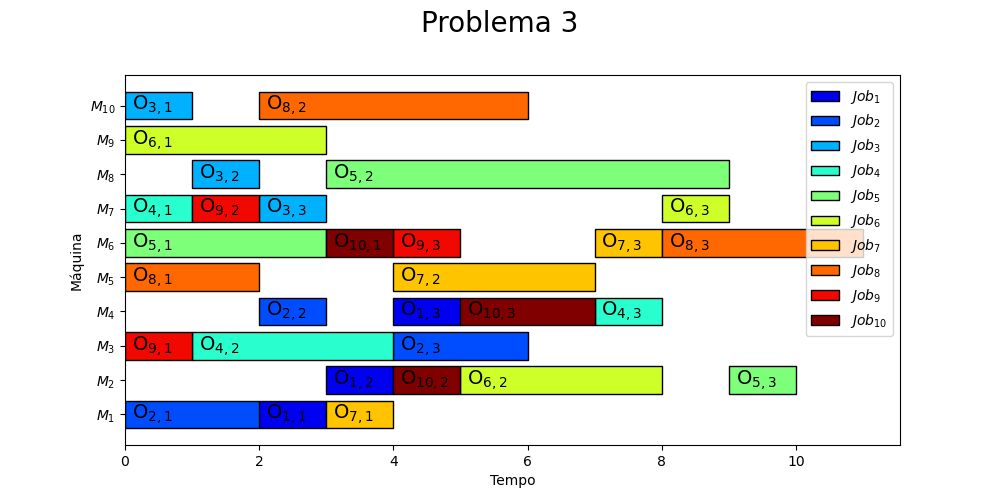
\includegraphics[width=\textwidth]{assets/solution_problem_3.png}
\end{figure}
%%%%%%%%%%%%%%%%%%
            
\noindent Nessa solução é possível observar que:
\begin{itemize}
    \item A máquina $M_1$ executa as operações $[O_{1,1}, O_{7,1}, O_{2,1}]$.
    \item Cada \textit{job} utiliza no mínimo duas máquinas para ser executado, como por exemplo o \textit{job} $J_1$ que é executado nas máquinas $[M_1 , M_3, M_4]$.
    \item O \textit{fitness} dessa solução é $7$.
\end{itemize}
%% Fim do [Solução] %%
%% 1 ::: Introdução
%% 1.1 ::: Problemas de Agendamento
%% 1.1.4 ::: FJSP
%% 1.1.4.2
%%\subsubsection{Cenários de Aplicação}
\indent O exemplo mais claro de aplicação do problema de \textit{Flexible Job Shop} é na produção industrial e em sistemas de manufatura, o que traz muito interesse econômico para encontrar boas soluções para essa categoria de problema.\\
%
\indent Como visto por \cite{Wari2016} nos tempos modernos onde existe uma grande competição e constantes mudanças e melhorias tecnológicas, a organização e otimização desses processos industriais se torna um gargalo a ser resolvido e pode ser um fator decisório no sucesso de uma indústria.
%% Fim do [Cenários de Aplicação] %%
%% Fim do [FJSP] %%
%% Fim do [Problemas de Agendamento] %%




%%%%%%%%%%%%%%%%%%%%%%%%%%%%%%%%%%%%%%%%%%%%%%%%%%%%%%%%%%%%%%%%%%%%%%%%%%%%%%%%%%%%%%%%%%%%%%%

%% 1 ::: Introdução
%% 1.2
\section{Soluções Existentes}
%% Interlúdio %%
Ao longo do tempo foram propostas, testadas, revisadas e aprimoradas diversas soluções para os problemas de agendamento, más como cada cenário de aplicação é único, não é possível definir que uma solução é melhor do que outra, pois isso depende dos critérios de analise de cada problema, contudo, durante o tempo algumas soluções chamaram a atenção de pesquisadores, seja por serem mais eficientes ou por serem mais adaptáveis a novas demandas, cenários e objetivos.\\
\indent Um tipo de solução muito recorrente são as soluções baseadas em comportamento biológico. 
%
Ao longo de milhões de anos a vida biológica no planeta Terra evoluiu e se adaptou para encontrar modos mais eficientes de resolver os diversos problemas que a natureza impõe. 
Então observando esses comportamentos adaptativos, foram propostos diversos algoritmos, 
como os algoritmos populacionais que simulam como populações de animais, como por exemplo, bandos de aves, enxames de abelhas ou colonias de formigas usam o comportamento de bando para solucionar um problema como o de encontrar alimento, ou fugir de predadores. 
Ou algoritmos que simulam as próprias regras de seleção natural para selecionar e evoluir indivíduos de uma população para gerar e acumular mutações afim de obter uma população de indivíduos mais adaptados e solucionar um problema, esses são os Algoritmos Genéticos e Algoritmos Evolutivos.\\
%% Fim do Interlúdio %%
%% 1 ::: Introdução
%% 1.2 ::: Soluções Existentes
%\subsection{Algoritmos Evolutivos}
\indent Os Algoritmos Evolutivos são baseados no mecanismo de seleção natural observado na natureza e descritos por Charles Darwin. Onde um individuo que tem alguma mutação que gere uma característica positiva que o destaque dos outros indivíduos da população, tem maior chance de se reproduzir e transmitir essa característica para os seus descendentes.\\

\noindent A estrutura básica de um Algoritmo Evolutivo é:
\begin{enumerate}
    \item Inicialização da população.
    \item Analise a qualidade de cada indivíduo.
    \item Selecionar os melhores indivíduos.
    \item Cruzar esses indivíduos melhores entre si, de modo a gerar uma nova população com melhores indivíduos.
    \item Voltar e repetir a partir do passo 2.
\end{enumerate}
Essa estrutura se repete até que seja atingido o critério de parada estabelecido pelo problema em questão.\\
\indent Além da estrutura básica é possível melhorar um Algoritmo Evolutivo através de um aprendizado continuo, ou seja, em um ambiente em que tenha mudanças constantes um Algoritmo Evolutivo pode se adaptar e assim se auto melhorar sem a necessidade de uma intervenção do programador.\\
%% Fim do [Alg EV] %%
%% 1 ::: Introdução
%% 1.2 ::: Soluções Existentes
%\subsection{Algoritmos Genéticos}
\indent Uma derivação dos Algoritmos Evolutivos são os Algoritmos Genéticos, utilizados para buscas e para otimizações, como nos problemas de escalonamento.\\
%
\indent Essa abordagem chama atenção por conseguir lidar com uma grande diversidade de soluções, o que a torna interessante especialmente em problemas de multi-objetivo como visto por \cite{Bagchi1999}.\\
\indent Os Algoritmos Genéticos são com certeza a abordagem mais utilizada dentre os Algoritmos Evolutivos, o que algumas vezes podem gerar a impressão de que Algoritmos Genéticos e Evolutivos são a mesma coisa, porém como o Algoritmo Genético lida com uma simulação de cromossomos isso o faz com que suas estruturas sejam muito mais dinâmicas, enquanto as técnicas de Algoritmos Evolutivos geralmente tem estruturas mais fixas.\\
%
\indent Para ter essa dinamicidade os Algoritmos Genéticos trabalham com o conceito de mutações aleatórias, que podem ou não serem boas para o indivíduo, porém por ser uma derivação dos Algoritmos Evolutivos o Algoritmo Genético conta também com os mecanismos de seleção e cruzamento entre indivíduos da população, o que tende a selecionar apenas os indivíduos com mutações que são positivas do ponto de vista do objetivo estabelecido pelo problema.\\
%% Fim do [GA] %%
%% 1 ::: Introdução
%% 1.2 ::: Soluções Existentes
%\subsection{Algoritmos Populacionais}
\indent Outra abordagem dos algoritmos bio inspirados são os Algoritmos Populacionais, nos quais normalmente não se é utilizado técnicas de evolução de indivíduos específicos, mas o foco é dado no comportamento da população. 
%
Seus cenários de aplicação vão além dos algoritmos de otimização e também são utilizados em algoritmos de busca e em efeitos visuais, sendo amplamente utilizada em filmes. 
%
Os Algoritmos Populacionais usam o conceito de inteligência de bando, onde indivíduos simples interagem entre si e com o ambiente e juntos convergem para uma solução. 
%
A inteligência de bando pode ser vista em diversos lugares da natureza, como em colonias de formigas, enxames de abelhas, na forma de voo migratório de aves, na forma de caça de aves predatórias como águias e na organização de cardumes de peixes. 
%
O que torna essa abordagem interessante é a sua característica decentralizada e de auto organização, o que a torna mais extensível e adaptável a cenários distribuídos. 
%
Um exemplo da utilização de Algoritmos Populacionais é na auto organização de drones e robôs, areá conhecida pelo nome de \textit{Swarm Robotics}. Fazendo assim com que caso algum robô tiver uma falha ou um defeito isso não afete a organização do grupo.\\
        
\noindent Dentre os principais algoritmos populacionais estão:
\begin{itemize}
    \item Otimização por Colonia de Formigas (\textit{Ant Colony Optimization}) 
    \item Difusão Estocástica de Busca (\textit{Stochastic Diffusion Search})
    \item Otimização por Enxame de Partículas (\textit{Particle Swarm Optimization})
\end{itemize}

\noindent Todos eles se baseiam em como a população de indivíduos encontram juntos um objetivo. Nesse trabalho é utilizado o algoritmo de Otimização por Enxame de Partículas (\textit{Particle Swarm Optimization}). 
%% Fim do [Algoritmos Populacionais] %%
%%
%% Fim do [Soluções Existentes] %%
%% 1 ::: Introdução
%% 1.3
\section{Particle Swarm Optimization — PSO}
%% Interlúdio %%
O algoritmo de Otimização por Enxame de Partículas ou PSO da sigla em inglês para (\textit{Particle Swarm Optimization}) é um algoritmo baseado nas teorias de inteligência de enxame. E diferentemente de outros algoritmos baseados em populações, como o \textit{Ant Colony Optimization} o \textit{Particle Swarm Optimization} é baseado em uma população genérica de indivíduos, embora sejam normalmente ilustrados como uma população de aves.\\
%% Fim do [Interlúdio] %%
%% 1 ::: Introdução
%% 1.3 ::: PSO
%% 1.3.1
%\subsection{Historia}
\indent O algoritmo \textit{Particle Swarm Optimization} foi proposto em 1995 por \cite{Kennedy1995} e desde então tem se mostrado muito promissor para a solução de diversos problemas de otimização. Por ser um algoritmo bem simples e flexível, ao longo do tempo já foram propostas varias variações para ele.\\
%
\indent O \textit{Particle Swarm Optimization} já foi alvo de várias discussões na área, pois alguns autores discordam de ele ser classificada como parte dos Algoritmos Evolutivos (areá da qual os Algoritmos Populacionais fazem parte), pois embora haja variações que sim, o \textit{Particle Swarm Optimization} básico não implementa mecanismos de seleção, cruzamento ou mutação, critérios básicos para a classificação como Algoritmo Evolutivo.
%
Atualmente o \textit{Particle Swarm Optimization} é classificado como parte da família dos algoritmos de \textit{Swarm Intelligence}.\\
%% Fim do [Historia] %%
%% 1 ::: Introdução
%% 1.3 ::: PSO
%% 1.3.2
%\subsection{Definição}
\indent A definição básica do algoritmo \textit{Particle Swarm Optimization} é uma população de partículas (também chamadas indivíduos), em que cada partícula tem uma velocidade e uma direção, além das informações da sua posição, qual é a qualidade de sua posição, qual foi a melhor posição na, qual ela já esteve, e acesso a um conhecimento compartilhado entre todos os indivíduos com a melhor posição em que qualquer um deles já esteve. E assim a cada rodada as partículas se movimentam com base na sua melhor posição e na melhor posição geral, e assim a cada rodada a população converge para uma solução ótima.\\
\indent As variáveis mais importantes do PSO são justamente as melhores posições, sendo a local normalmente chamada de $pBest$ e a geral normalmente chamada de $gBest$. Elas vão ser utilizadas para obter uma média que será a nova posição da partícula. Porém, existem resistências para que a partícula mude de direção, isso acontece por meio da inércia normalmente representada por $w$ que representa a força que tende a fazer a partícula seguir a direção onde ela já está se movendo. Essa força de inércia cresce conforme o valor de velocidade da partícula, normalmente representada por $v$, ou seja, partículas com uma maior velocidade $v$ tendem a tem uma maior inércia $w$.\\
\indent No \hyperref[alg:pso-base]{Pseudocódigo \ref{alg:pso-base}} 
é possível uma representação de um algoritmo PSO básico, esse algoritmo tem como base a formulação de \cite{martinez2009}.

\begin{figure}[h]
    \centering
    \small{Incluir o pseudo código de PSO básico aqui}
    \caption{Pseudocódigo de um PSO básico}
    \label{alg:pso-base}
\end{figure}

Na definição base do algoritmo não existe uma especificação de uma fórmula para o cálculo da movimentação da partícula. Porém, na 
\hyperref[fig:formula-movimentacao]{Formula \ref{fig:formula-movimentacao}} 
é possível ver uma representação de uma fórmula base para o cálculo de uma nova posição para a partícula.
        
\begin{figure}[ht]
    \centering
    \small{Incluir a Formula de movimentação aqui}
    \caption{Formula que define a movimentação da partícula}
    \label{fig:formula-movimentacao}
\end{figure}

%%
%% Fim do [Definição] %%


%% 1 ::: Introdução
%% 1.3 ::: PSO
%% 1.3.4
%\subsection{Problemas}
\indent Alguns cuidados devem ser tomados para a implementação do \textit{Particle Swarm Optimization} pois o algoritmo se mal configurado através dos parâmetros de velocidade, inercia e tamanho da população, tende a convergir prematuramente para uma solução não ótima, esse problema é normalmente chamado "Convergência Prematura".
%
Algumas medidas podem ser tomadas para diminuir essa possibilidade de convergência Prematura, como valores dinâmicos de inércia e uma ponderação nos valores de importância de $pBest$ e $gBest$.\\
%% Fim do [Problemas] %%
%% 1 ::: Introdução
%% 1.3 ::: PSO
%% 1.3.5
%\subsection{Melhorias}
%% Interlúdio %%
\indent Algumas técnicas podem ser usadas para melhorar o desempenho do PSO em cada cenário de aplicação. Porém, o efeito dessas abordagens varia de acordo com qual problema esta sendo resolvido e dos recursos e limitações de processamento e memoria do ambiente de processamento do algoritmo.\\
%% Fim do [Interlúdio] %%
%\subsubsection{Multithreading}
\indent Uma abordagem com bons resultados é o processamento distribuído do cálculo de movimentação de cada partícula como visto por \cite{Thongkrairat2019} e \cite{Kim2011}. Essa paralelização é possível graças a natureza distribuída dos algoritmos populacionais. No caso do PSO o único fator a se considerar para uma implementação distribuída é a atualização da variável $gBest$.\\
%
\indent Um exemplo de cenário onde se tem um bom proveito dessa abordagem são nos gerenciamentos de robôs e drones.\\  
%% Fim do [Multitheading] %%
%\subsubsection{Hibridização}
\indent Outra melhoria que tem demonstrado bons resultados é a hibridização de PSO com outros algoritmos, como com Algoritmos Genéticos como demostrado por \cite{carvalho2014}, ou com outros Algoritmos Evolutivos.
%
Essas abordagens de hibridizações com Algoritmos Evolutivos tendem a ser tão boas devido as características básicas do PSO como a de não ter componentes evolutivos em seus indivíduos, então uma adição de componentes evolutivos não atrapalha nenhum ponto do PSO.
%
Esses componentes evolutivos normalmente trabalham nos valores de inércia e de velocidade, criando partículas mais "teimosas" com uma tendência maior a fugir da convergência do grupo, o que pode ajudar a escapar de mínimos locais, evitando assim uma convergência prematura.
%
Um cenário que tem um bom proveito da hibridização evolutiva do PSO são os cenários com multi-objetivo, pois os componentes de mutação de Algoritmos Genéticos podem trazer uma maior diversidade para os indivíduos da população, gerando assim uma maior gama de exploração no espaço de soluções.\\
%% Fim do [Hibridização] %%
%\subsubsection{Dinamicidade}
\indent Outra abordagem promissora é a implementação de componentes dinâmicos na população, ou seja, que possam mudar suas características como velocidade e inercia de maneira dinâmica, por exemplo, se uma partícula perceber que esta longe do $gBest$ e está se movendo pouco ela pode reconhecer que possivelmente esta em um mínimo local e diminuir seu valor de inércia, ou aumentar o fator de importância do $gBest$.
%
Essa abordagem pode ser feita de maneira constante nas partículas, fazendo elas se atualizarem em tempo real.
%% Fim do [Dinamicidade] %%
%
%% Fim do [Melhorias] %%

%
%% Fim do [PSO] %%